\documentclass{article}
\usepackage{graphicx}
\usepackage{xcolor}
\usepackage{amsfonts}
\usepackage{amsmath}
\usepackage{amsthm}
\usepackage{geometry}
\usepackage{listings}
\lstset{
	basicstyle=\ttfamily,
	columns=fullflexible,
	frame=single,
	breaklines=true,
	postbreak=\mbox{\textcolor{red}{$\hookrightarrow$}\space},
}
\geometry{
	a4paper,
	total={170mm,257mm},
	left=20mm,
	top=20mm,
}
\newtheorem{theorem}{Theorem}[section]
\newtheorem{claim}[theorem]{Claim}


\begin{document}

\hfill\framebox{\parbox[t][5 true cm][c]{11 true cm}
{\hfil Space for project label}}

\begin{center}\LARGE\bf
CATAM: 9.3 Protein Comparison in Bioinformatics (8)
\end{center}

	\section{}
	\begin{claim}
		
	$ \forall i, j > 0 $
	\begin{equation}
		D(i, j) = min \{D(i-1, j) + 1, \; D(i, j-1) + 1, \; D(i-1, j-1) + s(S_i, T_j)\}
	\label{q1_eqn}	
	\end{equation}
	where $ s(S_i, T_j) = \begin{cases}
		1, & \text{if } S_i \neq T_j\\
		0, & \text{if } S_i = T_j 
	\end{cases}$
	\end{claim}

	\begin{proof}
		Assume $ i \leq m, \; j \leq n $. \\
		
		First, we defined two characters as 'aligned' if the operation done to edit them is either a 'Match' or 'Replace'. So if a character is not aligned with any other character, then it is 'Deleted' if the character is from S, and 'Inserted' if from T, since we are making edits on S.\\
		
		Consider the last elements $ S_i $ and $ T_j $ of string $ S[1, i] $ and $ T[1, j] $ respectively.\\
		if $ S_i $ and $ T_j $ are both aligned, they must be aligned to each other. Because If $ S_i $ is aligned to some letter other than $ T_j $, then $ T_j $ will not be aligned to any letter as $ S_i $ is the last character of S. Similarly in terms of the alignment of $ T_j $.\\
		Thus we have three cases:\\
		
		Case1: $ S_i $ and $ T_j $ are aligned to each other.\\
		If $ S_i = T_j $, then $ D(i, j) = D(i-1, j-1) $. Since $ S_i $ and $ T_j $ can be matched.\\
		If $ S_i \neq T_j $, then $ D(i, j) = D(i-1, j-1) + 1 $. Which means replacing $ S_i $ with $ T_j $.\\
		So $ D(i, j) = D(i-1, j-1) + s(S_i, T_j) $\\
		And $ s(S_i, T_j) = \begin{cases}
			1, & \text{if } S_i \neq T_j\\
			0, & \text{if } S_i = T_j 
		\end{cases}$\\
		Since if $ S_i \neq T_j $ then we need to Replace, which accounts for one edit operation, and otherwise if they match then there is no cost.
		
		Case2: $ S_i $ is not aligned.\\
		Then $ D(i, j) = \underbrace{D(i-1, j)}_\text{edits between $ S[1, i-1] $ and $ T[1, j] $} + \underbrace{1}_\text{deleting $ S_i $} $\\
		
		Case3: $ T_j $ is not aligned.\\
		Then $ D(i, j) = \underbrace{D(i, j-1)}_\text{edits between $ S[1, i-1] $ and $ T[1, j] $} + \underbrace{1}_\text{inserting $ T_j $} $\\
		
		If $ i > m $ or $ j > n $, then assume the characters after the last letter in strings S and T to be spaces, in which case the same cases apply.
		
		So $ D(i, j) $ has to equal one of these three cases, hence $ D(i, j) = min \{D(i-1, j) + 1, \; D(i, j-1) + 1, \; D(i-1, j-1) + s(S_i, T_j)\} $
		
		Use Boundary conditions $ D(0, 0) = 0 $, $ D(i, 0) = 1 $ and $ D(0, j) = j $.
	\end{proof}



	%question 2
	\section{}
	Refer to q2.py in Appendix (\ref{ap:q2}) for the program for this question.\\
	The edit distance is found to be 3.\\
	The order of operations is $ \mathcal{O} (mn) $.
	
	\section{}
	Refer to q3.py in Appendix (\ref{ap:q3}) for the program for this question.
	The edit distance is found to be 83, and the program outputs the first 50 steps of optimal alignment in Figure (\ref{fig:Q3_1}).\\
	
	\begin{figure}[h]
		\centering
		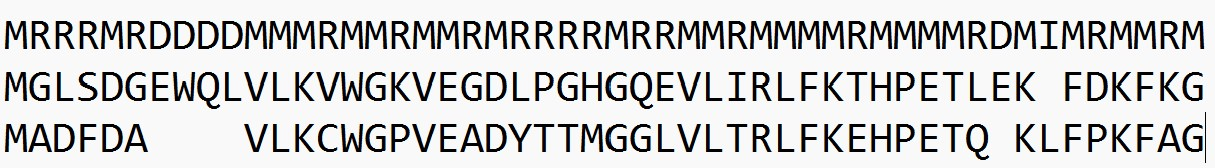
\includegraphics{figures/q3_1.jpg}
		\caption{first 50 alignment of protein A and B in second and third line resp.}
		\label{fig:Q3_1}
		
	\end{figure}

	\section{}
	
	Refer to q4.py in Appendix (\ref{ap:q4}) for the program for this question.
	The score v is found to be 290, and the program outputs the first 50 steps of optimal alignment for BLOSSUM scoring system in Figure (\ref{fig:Q4_1}).
	\begin{figure}[h]
		\centering
		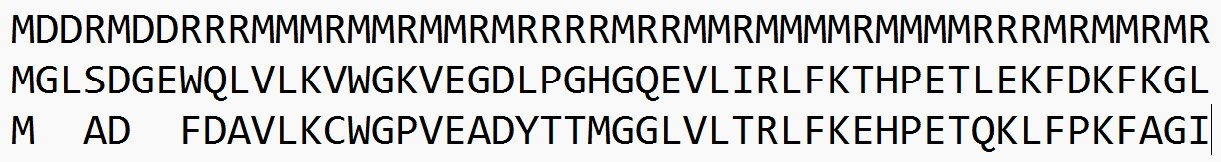
\includegraphics{figures/q4_1.jpg}
		\caption{first 50 alignment of protein A and B in second and third line resp. with BLOSSUM.}
		\label{fig:Q4_1}
		
	\end{figure}


	%question 5
	\section{}
	This is the SS-2 algorithm found from source [1], which finds all optimal paths with non-proportionally weighted gap scores.
	The specific scores in the algorithm are modified to fit our specifications. The changes include:
	\begin{enumerate}
		\item instead of minimizing the cost, we are maximising the score, hence many changes were made throughout to make 'min' into 'max', and in the initial conditions, any $ \inf $ is set instead to $ -\inf $.
		\item the weight $ w_l $ is taken to be a general $ u + vl $ in the source algorithm, but for our purposes $ w_l = u $ fixed for all $ l \geq 1 $
		%\item in the source, in the first double 'for' loops, the range is from (0 to m) and (0 to n), which I think is an error and I have changed it instead to (1 to m) and (1 to n).
	\end{enumerate}
	Refer to q5.py in Appendix (\ref{ap:q5}) for the implementation on first 10 characters of protein A and B.\\
	In this implementation, u is set to $ -12 $. The greatest alignment score is stored in R[m][n], which in this case has returned 2.
	For just the $v_{gap}$ score, steps 8 to 11 below for edge assignment is not needed. However edge assignment is useful for later questions when finding a specific alignment.
	The number labels for the algorithm is also in q5.py for ease of identification.\\
	First we look at a grid representing the two strings (see figures (\ref{fig:Q5_1}) and (\ref{fig:Q5_2})). Travelling diagonally in direction of 'D' means matching or replacing the corresponding letters, travelling vertically in direction of 'V' means deleting from S, and travelling horizontally in direction of 'H' means inserting into S from T.
	\begin{figure}[h]
		\centering
		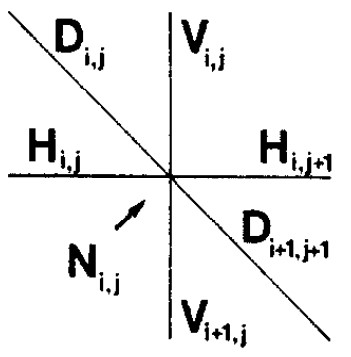
\includegraphics{figures/q5_1.jpg}
		\caption{direction of grid}
		\label{fig:Q5_1}
		
	\end{figure}

	\begin{figure}[h]
		\centering
		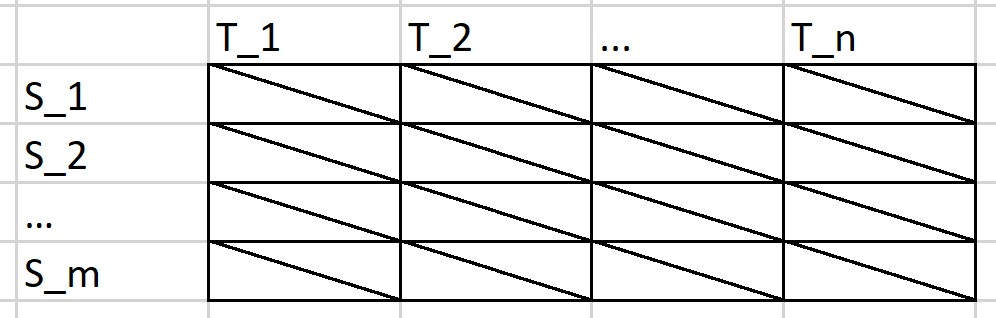
\includegraphics{figures/q5_2.jpg}
		\caption{direction of grid}
		\label{fig:Q5_2}
		
	\end{figure}
	
	Meaning for each variable:
	\begin{enumerate}
		\item (P, Q, R) store costs associated with node at each (i, j). Index i ranges from 0 to m and index j ranges from 0 to n. P, Q corresponds to costs of travelling in directions of V, H respectively. R represents the total alignment cost to that point.
		\item arrays $ (a_{i, j}, b_{i, j}, c_{i, j}, \dots, g_{i, j}) $ store data associated with graph edges V, H and D. Index i ranges from 0 to m+1 and Index j ranges from 0 to n+1. \\
		The specific meanings of the arrays before edge assignment starting on step 8 (note all paths start from (0, 0)):
		\begin{itemize}
			\item $ a_{i, j}, b_{i, j}, c_{i, j}$ equals 1 iff an optimal path to (i, j) uses $ V_{i, j}, H_{i, j} $ or $ D_{i, j} $ respectively.
			\item $ d_{i, j} $ and $ f_{i, j} $ equals 1 iff among paths to (i+1, j) through $ N_{i, j} $, an optimal one uses $ V_{i, j} $ and $ H_{i, j} $ respectively.
			\item $ e_{i, j} $ and $ g_{i, j} $ equals 1 iff among paths to (i+1, j) through $ N_{i, j} $, an optimal one does not use $ V_{i, j} $ and $ H_{i, j} $ respectively.
		\end{itemize}
		Meanings of the arrays after the edge assignment is complete:
		\begin{itemize}
			\item $ a_{i, j}, b_{i, j}, c_{i, j}$ equals 1 iff and optimal path to (m, n) uses $ V_{i, j}, H_{i, j} $ or $ D_{i, j} $ respectively;
			\item $ d_{i, j} = 1 $ iff every optimal path to (m, n) that uses $ V_{i, j} $ also uses $ V_{i-1, i} $;
			\item $ e_{i, j} = 1 $ iff every optimal path to (m, n) that uses $ V_{i, j} $ also uses $ V_{i+1, j} $.
			\item $ f_{i, j} = 1 $ iff every optimal path to (m, n) that uses $ H_{i, j} $ also uses $ H_{i, j-1} $;
			\item $ g_{i, j} = 1 $ iff every optimal path to (m, n) that uses $ H_{i, j} $ also uses $ H_{i, j+1} $
		\end{itemize}
		See figure (\ref{fig:Q5_3}) for a more graphical representation:
		
		
	\end{enumerate}

	\begin{figure}[h]
		\centering
		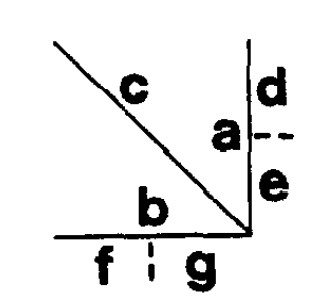
\includegraphics{figures/q5_3.jpg}
		\caption{graphical representation of arrays a, b, c, d, e, f, g}
		\label{fig:Q5_3}
	\end{figure}

	Algorithm SS-2:\\
	Step 1: set boundaries of the number and bit arrays:
	\begin{itemize}
		\item For j from 0 to n: $ P_{0, j} = - \infty $ and $ R_{0, j} = u $
		\item For i from 0 to m: $ Q_{i, 0} = - \infty $ and $ R_{i, 0} = u $
		\item $ R_{0, 0} = 0 $
		\item Set arrays a to g uniformly to 0
		\item $ C_{m+1, n+1} = 1 $
	\end{itemize}

	Cost Assignment:\\
	For i from 1 to m and j from 1 to n, execute steps 2 to 7:\\
	Step 2: Find the maximum score of path ending at $ N_{i, j} $ using edge $ V_{i, j} $:
	\begin{itemize}
		\item $ P_{i, j} = max(P_{i-1, j}, R_{i-1, j} + u) $
	\end{itemize}
	Step 3: Determine if cost $ P_{i, j} $ can be achieved using edge $ V_{i, j} $ and if it can be achieved without using edge $ V_{i-1, j} $:
	\begin{itemize}
		\item if $ P_{i, j} = P_{i-1, j} $: set $ d_{i-1, j} = 1 $
		\item if $ P_{i, j} = R_{i, j} + u $: set $ e_{i-1, j} = 1 $
	\end{itemize}
	Step 4: Find the maximum score of path ending at node $ N_{i, j} $ and using edge $ H_{i, j} $:
	\begin{itemize}
		\item $ Q_{i, j} = max(Q_{i, j-1}, R_{i, j-1} + u) $
	\end{itemize}
	Step 5: Determine if cost $ Q_{i, j} $ can be achieved using edge $ H_{i, j-1} $ and if it can be achieved without using edge $ H_{i, j-1} $:
	\begin{itemize}
		\item if $ Q_{i, j} = Q_{i, j-1} $: set $ f_{i, j-1} = 1 $
		\item if $ Q_{i, j} = R_{i, j-1} + u $: set $ g_{i, j-1} = 1 $
	\end{itemize}
	Step 6: Find the maximum score of a path ending at node $ N_{i, j} $:
	\begin{itemize}
		\item $ R_{i, j} = max(P_{i, j}, Q_{i, j}, R_{i-1, j-1} + s(S_i, T_i)) $
	\end{itemize}
	The scoring matrix in this case is taken to be BLOSSUM.\\
	Step 7: Determine if score $ R_{i, j} $ can be achieved by using edge $ V_{i, j}, \; H_{i, j}$ or $ D_{i, j} $:
	\begin{itemize}
		\item if $ R_{i, j} = P_{i, j} $: set $ a_{i, j} = 1 $
		\item if $ R_{i, j} = Q_{i, j} $: set $ b_{i, j} = 1 $
		\item if $ R_{i, j} = R_{i-1, j-1} + s(S_i, T_i) $: set $ c_{i, j} = 1 $
	\end{itemize}
	
	Edge Assignment: goes back into the arrays a to g and deletes paths which do not reach the end node (m, n).\\
	For i from m to 0 and j from n to 0, execute steps 8 to 11:\\
	Step 8: if there is no optimal path passing through node $ N_{i, j} $ which has cost $ R_{i, j} $ at node $ N_{i, j} $, remove edges $V_{i, j}, \; H_{i, j}$ and $ D_{i, j} $:
	\begin{itemize}
		\item if $ (a_{i+1,j} = 0 \; or \; e_{i, j} = 0) $ and $ (b_{i, j+1} = 0 \; or \; g_{i, j} = 0) $ and $ (c_{i+1,j+1} = 0) $: set $ a_{i, j}, \; b_{i, j} $ and $ c_{i, j} $ to 0
	\end{itemize}
	Step 9: if no optimal path passes through $ N_{i, j} $, proceed to next node:
	\begin{itemize}
		\item if $ a_{i+1, j} = b_{i, j+1} = c_{i+1, j+1} = 0 $: skip steps 10 to 11.
	\end{itemize}
	Step 10: if edge $ V_{i+1, j} $ is in an optimal path and requires edge $ V_{i, j} $ to be in an optimal path, determine if an optimal path that uses edge $ V_{i+1, j} $ must use edge $ V_{i, j} $ and the converse:
	\begin{itemize}
		\item if $ a_{i+1, j} = 1 $ and $ d_{i, j} = 1 $: set $ d_{i+1, j} = 1-e_{i, j} $, set $ e_{i, j} = 1-a_{i, j} $ and set $ a_{i, j} = 1 $. Otherwise: set $ d_{i+1, j} $ and $ e_{i, j} $ to 0
	\end{itemize}
	Step 11: if edge $ H_{i, j+1} $ is an optimal path and requires edge $ H_{i, j} $ to be in an optimal path, determine if an optimal path that uses edge $ H_{i, j+1} $ must use edge $ H_{i, j} $ and the converse:
	\begin{itemize}
		\item If $ b_{i, j+1} = 1 \; and \; f_{i, j} = 1 $: set $ f_{i, j+1} = 1-g_{i, j} $, set $ g_{i, j} = 1-b_{i, j} $ and set $ b_{i, j} = 1 $. Otherwise: set $ f_{i, j+1} $ and $ g_{i, j} $ to 0
	\end{itemize}

	Arrays a to g represents all possible optimal paths from (0,0) to (m, n) with score 2. a, b and c represent all edges in possible optimal paths, but within contains possible non-optimal paths, which we can disern from d, e, f, g.\\
	
	This algorithm has complexity $ \mathcal{O}(mn) $ since there are a fixed number of steps for each node $ N_{i, j} $ and there are mn nodes.\\
	The boundary conditions are indicated in Step 1, where entries in first row of P and first column of Q are set to negative infinity so it has a lower score than any other number. First row and column of R is set to u because travelling just horizontally or just vertically would indicate just leaving a gap, which will always have score of u. $ c_{m+1, n+1} $ is initially set to 1 so steps 8 and 9 are false for node $ N_{m, n} $, since if it was true then all elements of a, b, c will be reassigned as 0.
	
	%question 6: Done, but needs double checking
	\section{}
	Refer to q6.py in Appendix (\ref{ap:q6}) for the program for this question.\\
	u is set to -12, protein C and D are compared.
	q6.py Implements the algorithm specified in question 5, and adds a few more functions to choose one specific optimal path to print out one possible optimal alignment in figure (\ref{fig:Q6_1}). The program also outputs the final score $ v_{gap} $ which was stored in $ R_{m, n} $ as 1236.
	
	\begin{figure}[h]
		\centering
		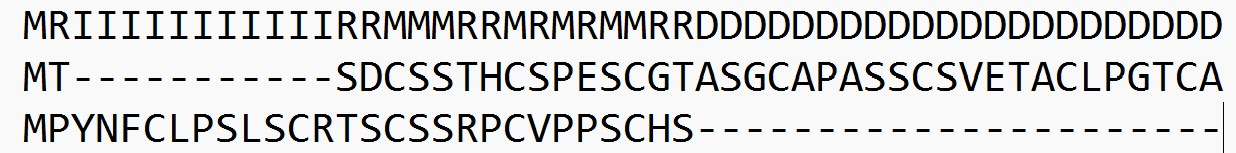
\includegraphics{figures/q6_1.jpg}
		\caption{first 50 alignment of protein C and D example from SS-2}
		\label{fig:Q6_1}
		
	\end{figure}
	
	%question 7
	\section{}
	Claim:\\
	$\stackrel{lim}{n \rightarrow \infty}\, inf\, \mathbb{E}(\frac{v_{gap}(U^n, V^n)}{n}) > 0 $\\
	Proof:\\
%	If $ p = 0 $ or $ p = 1 $, then both sequences are perfectly matched as there is only one possible letter, so $ v_{gap}(U^n, V^n) = n \Rightarrow \stackrel{lim}{n \rightarrow \infty} \, inf \,  \mathbb{E}(\frac{v_{gap}}{n}) = 1 > 0 $. Then we are done.\\
%	So now assume p is not 0 or 1.\\
	Writing $ U_i' $, $ V_i' $ as the $ i $th element of $ U^n $ and $ V^n $ after alignment respectively, then we can write $ v_{gap} $ as follows:
	\[v_{gap}(U^n, V^n) = max(\sum s(U_i', V_i') + u \times \# gaps)\]
	The best case senario is if all the n letters match with a score of 1, and since we are taking the maximum, the score must be better than $\sum_{i = 1}^{n} S(U_i, V_i)$. So:
	\[1 \geq \frac{v_{gap}(U^n, V^n)}{n} \geq \frac{\sum_{i = 1}^{n} S(U_i, V_i)}{n}\]
	If $ \frac{v_{gap}(U^n, V^n)}{n} $ is within these bounds then the expectation must be within these bounds as well.
	Since $ \mathbb{P}(s(U_i, V_i) = 1) = p^2 + (1-p)^2 $ and $ \mathbb{P}(s(U_i, V_i) = -1) = 2p(1-p) $, as $ n \rightarrow \infty $, $ \inf \frac{\sum_{i = 1}^{n} S(U_i, V_i)}{n} \rightarrow p^2 + (1-p)^2 - 2p(1-p) = (2p-1)^2$, which is greater than zero if p is not $ 1/2 $.\\
	So if $ p \neq 1/2 $, 
	\[1 \geq \stackrel{lim}{n \rightarrow \infty} \, inf \, \mathbb{E} (\frac{v_{gap}(U^n, V^n)}{n}) \geq (2p-1)^2 > 0\]
	Therefore limit is finite and is greater than 0, so we are done.
	
	For $ p = 1/2 $, the limit of the lower bound from above approaches 0, so we need to find an alignment better than leaving no gaps. Consider the case when $ |u| $ consecutive letters are different. Since in this case $ \mathbb{P}(s(U_i, V_i) = -1) = 1/2 $, the probability that $ |u| $ consecutive letters are different is $ k = (1/2)^{|u|} $. In this case, if no gap is left then at least $ u $ is added to the gap score. It is more effective to find the next letter in V which matches the first letter of this size $ |u| $ sequence in U, then the score added is $ u + 1 $, which means at least a score of 1 is added to the gap score of when no gap is left.\\
	For n large:
	
	\[\Rightarrow v_{gap}(U^n, V^n) = max(\sum s(U_i', V_i') + u \times \# gaps) \geq \sum_{i = 1}^{n} S(U_i, V_i) + k \times (n/|u|)\]
	
	Where there are at least $ n/|u| $ sections of length $ |u| $ in a sequence of length n.
	
	\[\Rightarrow 1 \geq \stackrel{lim}{n \rightarrow \infty} \, inf \, \mathbb{E} (\frac{v_{gap}(U^n, V^n)}{n}) \geq 0 + k/|u| > 0\]
	
	
	
	%question 8
	\section{}
	Refer to q8.py and GGP.py in Appendix (\ref{ap:q8}) and (\ref{ap:GGP}) for the program for this question.
	
	This program takes $ u = -3, \; p = \frac{1}{2} $ and returns an estimated $ n^{-1} \mathbb{E}(v_{gap}(U^n, V^n)) $, which we will just call E.
	Intuitively, the larger the sample size, the more accurately the result will tend to the true result.
	Through experimentation, I have also found the result is more accurate the longer the possible protein: see results from a few different lengths for sample size 100 in figure (\ref{fig:Q8_2})\\
	%in this figure, need a few results for each different length to show how much they vary.
	So since by length 1210, the data does not vary at the 2 d.p. level, I assume at least this accuracy for longer proteins.\\
	The result I arrive at is 0.43.
	Finding the result of proteins for length increasing by 20 each time, I plot a graph of length against E in figure (\ref{fig:Q8_1}), and the blue dotted line indicates the E = 0.43 line, which seems plausible as the limit of the data as n increases.
	
	\begin{figure}[h]
		\centering
		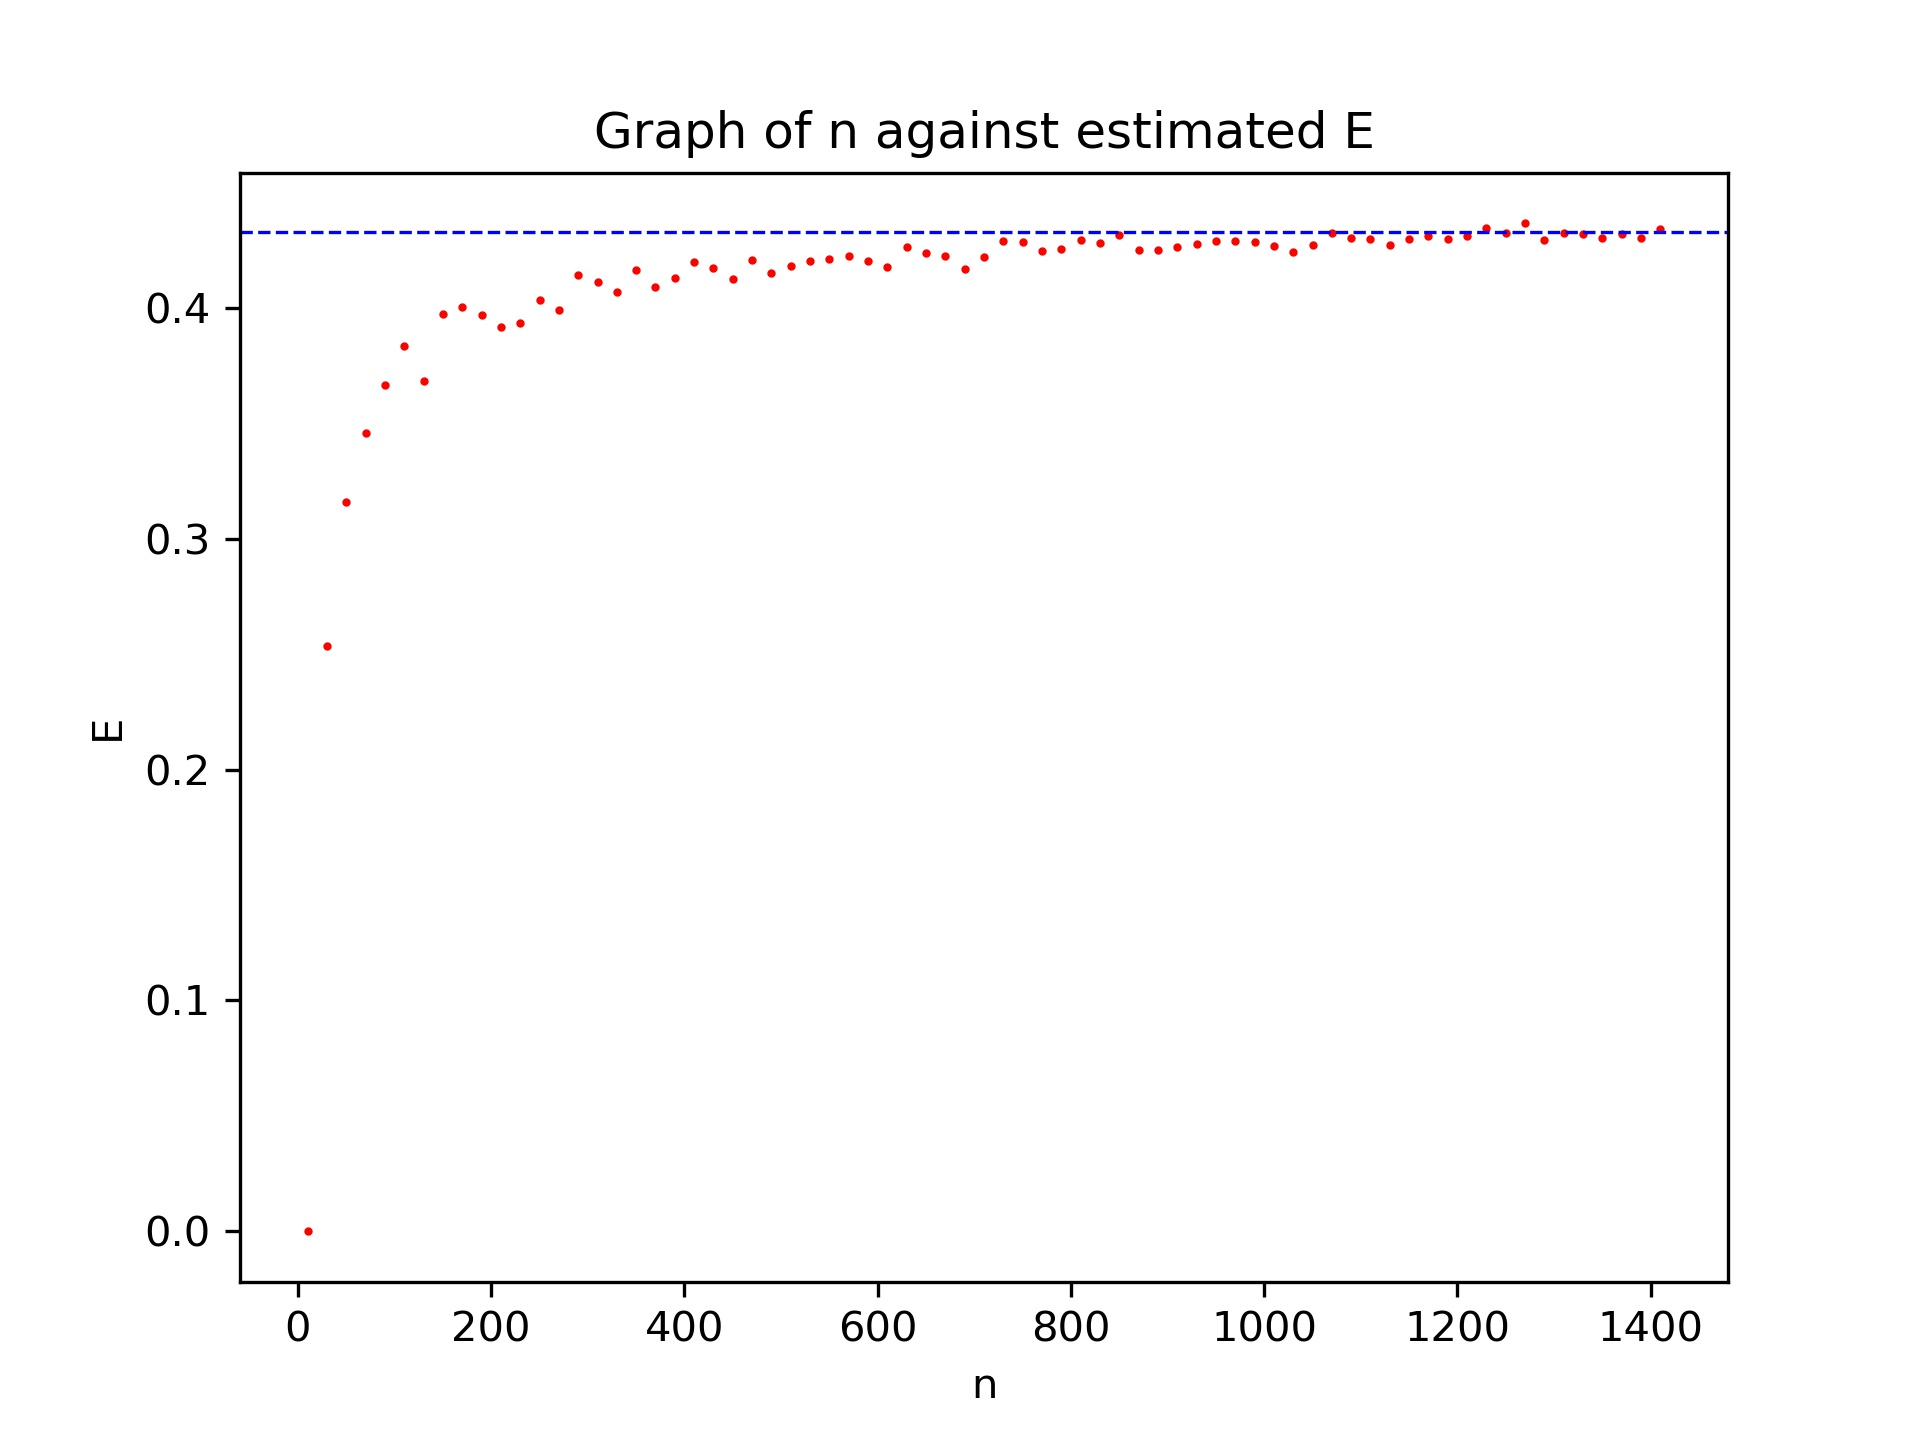
\includegraphics{figures/q8_1.jpg}
		\caption{Graph of E calculated with q8.py with corresponding length of string n}
		\label{fig:Q8_1}
	\end{figure}
	
	%data from program with 
	\begin{figure}[h]
		\centering
		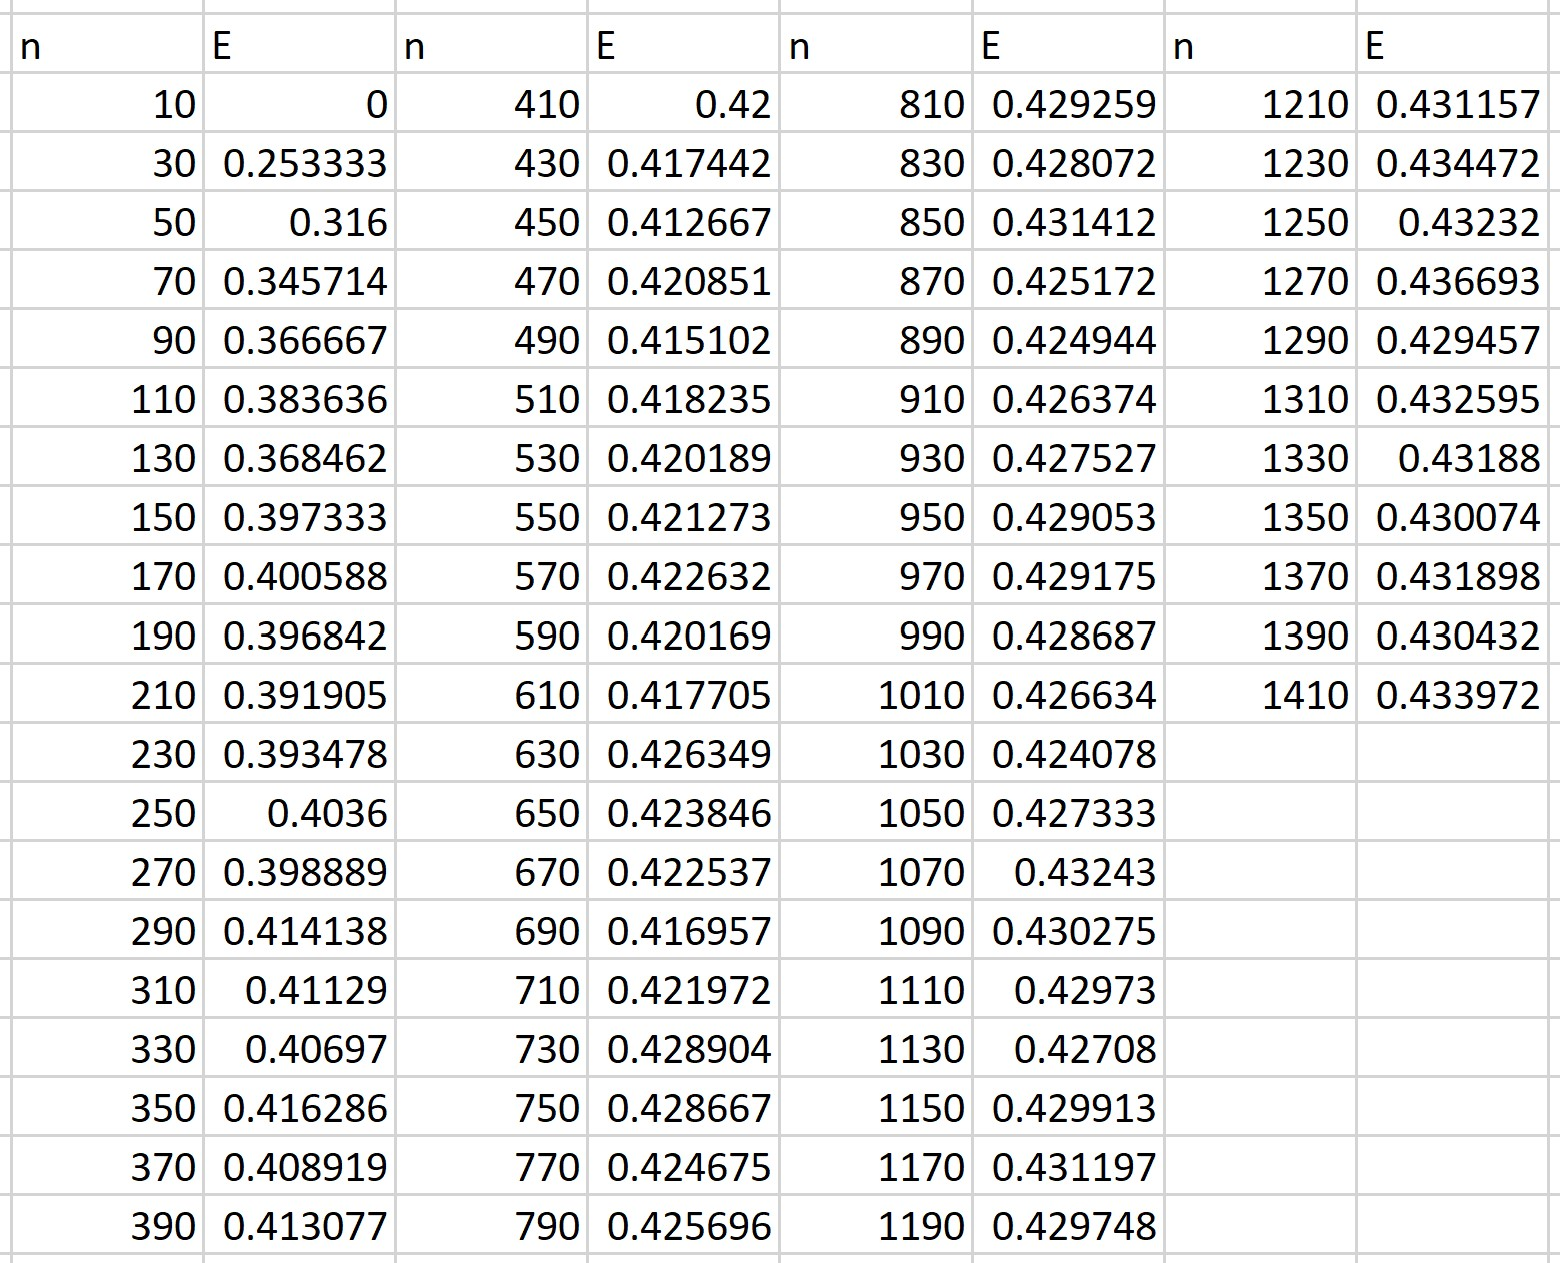
\includegraphics{figures/q8_2.jpg}
		\caption{E calculated with q8.py with corresponding length of string n}
		\label{fig:Q8_2}
	\end{figure}
	
	
	%%%%%%%%%%%%%%%%
	%insert figure
	
	
	
	%Question 9: done, but needs to be double checked
	\section{}
	For any string $ X $, let $ X' $ be any prefix of X (i.e. $ X' = X[1, x] $ for some integer x less than the length of X). Let $ X'' $ be any suffix of X (i.e. $ X'' = X[y, n] $ for any $ y \leq n $, where n is the length of X).
	
	\begin{claim}
		 \begin{equation}
		 	v_{sub} = max\{v_{sfx}(S', T')\} 
		 \label{q9_eqn}
		 \end{equation}
		where $ v_{sub} = max\{v(\hat{S}, \hat{T})|\hat{S}, \hat{T} \text{ substrings of S and T resp.}\} $ and $ v_{sfx} = max\{v(S'', T'')\} $.
	\end{claim}

	\begin{proof}
		\begin{align}
			RHS & = max\{v_{sfx}(S', T')\}\\
			& = max\{max\{v((S')'', (T')'')\}\}
		\end{align}
		Max of the max of sets of elements is equal to the max of all elements in the sets, so we need to show $ max \{v((S')'', (T')'')\} = max\{v(\hat{S}, \hat{T})\} $\\
		which is equivalent to showing $ \{((S')'', (T')'')\} $ contains all substring pairs of S and T.\\
		
		S' includes all substrings $ S[1, a] $ for any $ a < m $ and T' includes all substrings $ T[1, b] $ for any $ b < n $, so (S')'' can be any substring $ S[c, a] $ for any $ c<a<m $ and (T')'' can be any substring $ T[d, b] $ for any $ d < b < n $. Therefore for any $ a, b, c, d > 0$ such that $ c<a<m $ and $ d<b<n $, $ (S[c, a], T[d, b]) \in \{((S')'', (T')'')\} $, and any element of $\{((S')'', (T')'')\} $ must be limited to substring pairs of S and T by definition.
	\end{proof}

	%question 10
	\section{}
	We know that $ V_{sfx}(i, j) = v_{sfx}(S[1, i], T[1, j]) = max \{v(S[1, i]', T[i, j]')\} = max\{v(S[a, i], T[b, j])| a \leq i, \; b \leq j\} $.
	If either a or b are equal to i or j respectively, then one of the strings will be empty. In this case $ V_{sfx}(i, j) = max\{v(S[a, i], T[b, j])\} = 0 $, because since $ s(a, -) = s(-, a) \leq 0 $, if one substring is empty, if the other substring is non-empty then the score will always be negative, so both substrings must be empty, then the maximum score is 0.
	If we then assume $ a < i $ and $ b < j $, there are 3 cases similar to question 1 (since $ S_i $ and $ T_j $ must either be aligned to each other, or one of them is not aligned):\\
	Case 1: $ S_i $ and $ T_j $ are aligned to each other.\\
	The $ V_{sfx}(i, j) = \underbrace{V_{sfx}(i-1, j-1)}_\text{max score aligning substrings excluding $ S_i $ and $ T_j $} + \underbrace{s(S_i, T_j)}_\text{score aligning $ S_i $ and $ T_j $}$\\
	Case 2: $ S_i $ is not aligned.\\
	Then $ V_{sfx}(i, j) = \underbrace{V_{sfx}(i-1, j)}_\text{max score aligning substrings excluding $ S_i $ from S} + \underbrace{s(S_i, -)}_\text{deleting $ S_i $} $\\
	Case3: $ T_j $ is not aligned.\\
	Then $ V_{sfx}(i, j) = \underbrace{V_{sfx}(i, j-1)}_\text{max score aligning substrings excluding $ T_j $ from T} + \underbrace{S(-, T_j)}_\text{inserting $ T_j $} $\\
	
	Since these contain all possible cases and $ V_{sfx} $ is by definition the maximum possible score, 
	\[V_{sfx}(i, j) = \begin{cases}
		0, \\
		V_{sfx}(i-1, j-1) + s(S_i, T_j),\\
		V_{sfx}(i-1, j) + s(S_i, -),\\
		V_{sfx}(i, j-1) + s(-, T_j),
	\end{cases}\]

	If i or j are 0, the $ V_{sfx} $ is also 0, since one of the string will definitely be empty, so the maximum score is achieved when the other is also empty, by same reasoning as when $ a = i $ or $ b = j $ at the beginning of this question.
	
	%question 11
	\section{}
	Refer to q11.py in Appendix (\ref{ap:q11}) for the program for this question.
	BLOSUM from question 4 is used, and cost of deleting and inserting is set to -2. 
	For proteins C and D, $ v_{sub} $ returns as 283, which is outputted in q11.py.
	
	\newpage
	\begin{center}\LARGE\bf
		References
	\end{center}
	[1]Altschul, Stephen \& Erickson, Bruce. (1986). Optimal sequence alignment using affine gap costs. Bulletin of mathematical biology. 48. 603-16. 10.1007/BF02462326. 
	
	\newpage
	
	\appendix
	\centering\textbf{\huge Appendix}
	\section{q2.py}
	\label{ap:q2}
	\begin{lstlisting}[language = python]
def edit_distance(s, t):
	I = len(s) + 1
	J = len(t) + 1
	D = [[0 for i in range(J)] for j in range(I)]

for i in range (I):
	D[i][0] = i

for j in range(J):
	D[0][j] = j

for i in range(1, I):
for j in range(1, J):
	m1 = D[i-1][j] + 1
	m2 = D[i][j-1] + 1
	m3 = D[i-1][j-1] + compare(s[i-1], t[j-1])
	D[i][j] = min([m1, m2, m3])
	
	return D[len(s)][len(t)]

def compare(a, b):
	if a == b:
	return 0
	else:
	return 1

def main():
	ed = edit_distance('shesells', 'seashells')
	print(ed)


if __name__ == '__main__':
main()
	\end{lstlisting}

	\section{q3.py}
	\label{ap:q3}
	\begin{lstlisting}[language = python]
import numpy as np

def edit_distance(s, t):
I = len(s) + 1
J = len(t) + 1
D = [[0 for i in range(J)] for j in range(I)]
path = [[[0, 0] for i in range(J)] for j in range(I)]

for i in range (I):
D[i][0] = i

for j in range(J):
D[0][j] = j

for i in range(1, I):
for j in range(1, J):
m1 = D[i-1][j] + 1
m2 = D[i][j-1] + 1
m3 = D[i-1][j-1] + compare(s[i-1], t[j-1])
D[i][j] = min([m1, m2, m3])
index = np.argmin([m1, m2, m3])

if index == 0:
path[i][j] = [i-1, j]
elif index == 1:
path[i][j] = [i, j-1]
else:
path[i][j] = [i-1, j-1]

#-----------ignore -------------------------------
# if index == 0:
#     edit_seq = edit_seq + 'D'
#     salign = salign + s[i-1]
#     talign = talign + ' '

# elif index == 1:
#     edit_seq = edit_seq + 'I'
#     salign = salign + ' '
#     talign = talign + t[i-1]
# else:
#     if compare(s[i-1], t[j-1]) == 0:
#         edit_seq  = edit_seq + 'M'
#     else:
#         edit_seq = edit_seq + 'R'
#     salign = salign + s[i-1]
#     talign = talign + t[i-1]
#-------------------------------------------------------


align_path(path, s, t)
return D[len(s)][len(t)], D, path

def align_path(P, s, t):
edit_seq = ''
salign = ''
talign = ''
current = [len(s), len(t)]
count = 0
while current != [0, 0] and count < 500:
count += 1
if P[current[0]][current[1]] == [current[0]-1, current[1]-1]:
if s[current[0]-1] == t[current[1]-1]:
edit_seq = 'M' + edit_seq

else:
edit_seq = 'R' + edit_seq
salign = s[current[0]-1] + salign
talign = t[current[1]-1] + talign
current = list(np.subtract(np.array(current), np.array([1, 1])))
elif P[current[0]][current[1]] == [current[0]-1, current[1]]:
edit_seq = 'D' + edit_seq
salign = s[current[0]-1] + salign
talign = ' ' + talign
current = list(np.subtract(np.array(current), np.array([1, 0])))
else:
edit_seq = 'I' + edit_seq
salign = ' ' + salign
talign = t[current[1]-1] + talign
current = list(np.subtract(np.array(current), np.array([0, 1])))
print(edit_seq[:50])
print(salign[:50])
print(talign[:50])



def compare(a, b):
if a == b:
return 0
else:
return 1

def main():
file = open('proteins.txt', "r")
content = file.readlines()
content = [line.rstrip() for line in content]
#print(content)

proteinA = content[1]
proteinB = content[3]

ed, D, P = edit_distance(proteinA, proteinB)
#ed, D, P = edit_distance('shesells', 'seashellsa')

print()

if __name__ == '__main__':
main()
	\end{lstlisting}

	\section{q4.py}
	\label{ap:q4}
	\begin{lstlisting}[language=python]
import numpy as np

with open('blosum.txt', 'r') as f:
blosum = [[num for num in line.split()] for line in f]


def edit_distance(s, t):
I = len(s) + 1
J = len(t) + 1
D = [[0 for i in range(J)] for j in range(I)]
path = [[[0, 0] for i in range(J)] for j in range(I)]

for i in range (I):
D[i][0] = i*(-8)

for j in range(J):
D[0][j] = j*(-8)

for i in range(1, I):
for j in range(1, J):
m2 = D[i-1][j] -8
m1 = D[i][j-1] -8
m3 = D[i-1][j-1] + score(s[i-1], t[j-1])
D[i][j] = max([m1, m2, m3])
index = np.argmax([m1, m2, m3])

if index == 0:
path[i][j] = [i, j-1]
elif index == 1:
path[i][j] = [i-1, j]
else:
path[i][j] = [i-1, j-1]    
align_path(path, s, t)
return D[len(s)][len(t)], D, path

def align_path(P, s, t):
edit_seq = ''
salign = ''
talign = ''
current = [len(s), len(t)]
count = 0
while current != [0, 0] and count < 500:
count += 1
if P[current[0]][current[1]] == [current[0]-1, current[1]-1]:
if s[current[0]-1] == t[current[1]-1]:
edit_seq = 'M' + edit_seq

else:
edit_seq = 'R' + edit_seq
salign = s[current[0]-1] + salign
talign = t[current[1]-1] + talign
current = list(np.subtract(np.array(current), np.array([1, 1])))
elif P[current[0]][current[1]] == [current[0]-1, current[1]]:
edit_seq = 'D' + edit_seq
salign = s[current[0]-1] + salign
talign = ' ' + talign
current = list(np.subtract(np.array(current), np.array([1, 0])))
else:
edit_seq = 'I' + edit_seq
salign = ' ' + salign
talign = t[current[1]-1] + talign
current = list(np.subtract(np.array(current), np.array([0, 1])))
print(edit_seq[:50])
print(salign[:50])
print(talign[:50])



def score(a, b):
indexa = blosum[0].index(str(a))
indexb = blosum[0].index(str(b))
return int(blosum[indexa][indexb])

def main():
# some changes were made to protein and blossum files to make reading them easier
# contrary to before, now the higher the score, the better the alignment.
file = open('proteins.txt', "r")
content = file.readlines()
content = [line.rstrip() for line in content]
file.close()



#print(content)

proteinA = content[1]
proteinB = content[3]

v, D, P = edit_distance(proteinA, proteinB)


print()

if __name__ == '__main__':
main()
	\end{lstlisting}
	
	\section{q5.py}
	\label{ap:q5}
	\begin{lstlisting}[language = python]
#derived from source [1], a better version of Gotoh and Taylor's algorithm with O(mn) complexity and affine gap costs
#uses many different edge options to map out path
#The original algorithm takes w_k = v + uk, here we would take u to be 0, and v to be some fixed value
#This algorithm is called SS-2


from cmath import inf
import numpy as np

def score(x, y):
    indexx = blosum[0].index(str(x))
    indexy = blosum[0].index(str(y))
    return int(blosum[indexx][indexy])


with open('blosum.txt', 'r') as f:
    blosum = [[num for num in line.split()] for line in f]


file = open('proteins.txt', "r")
content = file.readlines()
content = [line.rstrip() for line in content]
file.close()
proteinA = content[1][0:9]
proteinB = content[3][0:9]

u = -12 #constant gap penalty
s = proteinA
t = proteinB
J = len(t)+1
I = len(s)+1

#[1]
P = [[0 for j in range(J)]for i in range(I)]
R = [[0 for j in range(J)]for i in range(I)]
Q = [[0 for j in range(J)]for i in range(I)]

a = [[0 for j in range(J+1)]for i in range(I+1)]
b = [[0 for j in range(J+1)]for i in range(I+1)]
c = [[0 for j in range(J+1)]for i in range(I+1)]
d = [[0 for j in range(J+1)]for i in range(I+1)]
e = [[0 for j in range(J+1)]for i in range(I+1)]
f = [[0 for j in range(J+1)]for i in range(I+1)]
g = [[0 for j in range(J+1)]for i in range(I+1)] #setting all bit arrays to 0
for j in range(J):
    P[0][j] = -inf
    R[0][j] = u
for i in range(I):
    Q[i][0] = -inf
    R[i][0] = u

R[0][0] = 0
c[I][J] = 1



for i in range(1, I):
    for j in range(1, J):
        #[2]: find max cost of path ending at N[i][j] using edge V[i][j]
        P[i][j] = max([P[i-1][j], R[i-1][j] + u])
        #[3]:
        if P[i][j] == P[i-1][j]:
            d[i-1][j] = 1

        if P[i][j] == R[i-1][j] + u:
            e[i-1][j] = 1

        #[4]: find max cost of path ending at N[i][j] using edge H[i][j]
        Q[i][j] = max(Q[i][j-1], R[i][j-1] + u)
        #[5]:
        if Q[i][j] == Q[i][j-1]:
            f[i][j-1] = 1
        if Q[i][j] == R[i][j-1] + u:
            g[i][j-1] = 1

        #[6]:
        R[i][j] = max([P[i][j], Q[i][j], R[i-1][j-1] + score(s[i-1], t[j-1])])
        #[7]:
        if R[i][j] == P[i][j]:
            a[i][j] = 1
        if R[i][j] == Q[i][j]:
            b[i][j] = 1
        if R[i][j] == R[i-1][j-1] + score(s[i-1], t[j-1]):
            c[i][j] = 1

#----------edge assignment-------------
for i in reversed(range(I-1)):
    for j in reversed(range(J-1)):
        #[8]: if there is no optimal path passing through node N[i][j] which has cost R[i][j]
        #at node N[i][j], remove edges V[i][j], H[i][j] and D[i][j]
        if (a[i+1][j] == 0 or e[i][j] == 0) and (b[i][j+1] == 0 or g[i][j] == 0) and (c[i+1][j+1] == 0):
            a[i][j] = 0
            b[i][j] = 0
            c[i][j] = 0

        #[9]: if there exists optimal path passing through node N[i][j]
        if not (a[i+1][j] == 0 and b[i][j+1] == 0 and c[i+1][j+1] == 0):
            #[10]: if V[i+1][j] is an optimal path and requires edge V[i][j] to be in an optimal path, determine if an optimal path that uses edge V[i+1][j] must use edge V[i][j] and the converse:
            if a[i+1][j] == 1 and d[i][j] == 1:
                d[i+1][j] = 1-e[i][j]
                e[i][j] = 1-a[i][j]
                a[i][j] = 1
            else:
                d[i+1][j] = 0
                e[i][j] = 0

            #[11]: if edge H[i][j+1] is in an optimal path and requires edge H[i][j] to be in an optimal path, determine if an optimal path that uses edge H[i][j+1] must use edge H[i][j] and the converse:
            if b[i][j+1] == 1 and f[i][j] == 1:
                f[i][j+1] = 1-g[i][j]
                g[i][j] = 1-b[i][j]
                b[i][j] = 1
            else:
                f[i][j+1] = 0
                g[i][j] = 0
	\end{lstlisting}
	
	\section{q6.py}
	\label{ap:q6}
	\begin{lstlisting}[language=python]
###############################
#copy of q5 with mapping and score calculating
###############################


#derived from source [1], a better version of Gotoh and Taylor's algorithm with O(mn) complexity and affine gap costs
#uses many different edge options to map out path
#The original algorithm takes w_k = v + uk, here we would take u to be 0, and v to be some fixed value
#This algorithm is called SS-2


from cmath import inf
import numpy as np

from q4 import edit_distance


with open('blosum.txt', 'r') as f:
blosum = [[num for num in line.split()] for line in f]


file = open('proteins.txt', "r")
content = file.readlines()
content = [line.rstrip() for line in content]
file.close()

#currently set to first 5 letters, needs to be changed to protein C and D
proteinC = content[5]
proteinD = content[7]

u = -12 #constant gap penalty
s = proteinC
t = proteinD


# #test for 8
# u = -3
# blosum = [['#', 'a', 'b'], ['a', '1', '-1'], ['b', '-1', '1']]
# s = 'ababbabbaababbaabbbababbaabbbb'
# t = 'bbbaabbbbbbbbaabbaabaaaabbbaba'

#######################
J = len(t)+1
I = len(s)+1
P = [[0 for j in range(J)]for i in range(I)]
R = [[0 for j in range(J)]for i in range(I)]
Q = [[0 for j in range(J)]for i in range(I)]

a = [[0 for j in range(J+1)]for i in range(I+1)]
b = [[0 for j in range(J+1)]for i in range(I+1)]
c = [[0 for j in range(J+1)]for i in range(I+1)]
d = [[0 for j in range(J+1)]for i in range(I+1)]
e = [[0 for j in range(J+1)]for i in range(I+1)]
f = [[0 for j in range(J+1)]for i in range(I+1)]
g = [[0 for j in range(J+1)]for i in range(I+1)] #setting all bit arrays to 0
for j in range(J):
P[0][j] = -inf
R[0][j] = u
for i in range(I):
Q[i][0] = -inf
R[i][0] = u

R[0][0] = 0
c[I][J] = 1

def score(x, y):
if x != ' ':
indexa = blosum[0].index(str(x))
indexb = blosum[0].index(str(y))
return int(blosum[indexa][indexb])
else:
return 0

#----one possible alignment------------------
def create_path(a, b, c, d, e, f, g):
current = [0, 0]
count = 0
prev = ''
#stores whether previous step in path is up or left
path = [[[0, 0] for i in range(J+1)] for j in range(I+1)]
while current != [len(s), len(t)] and count < 500:

#for debugging:
A = a[current[0]+1][current[1]]
B = b[current[0]][current[1]+1]
C = c[current[0]+1][current[1]+1]
D = d[current[0]+1][current[1]]
E = e[current[0]+1][current[1]]
F = f[current[0]][current[1]+1]
G = g[current[0]][current[1]+1]


count += 1
if c[current[0]+1][current[1]+1] == 1:
path[current[0]][current[1]] = [current[0]+1, current[1]+1]
current = [current[0]+1, current[1]+1]
prev = 'd'
elif (a[current[0]+1][current[1]] == 1) and (count == 0 or (not (d[current[0]+1][current[1]] == 0 and  prev == 'v')and not (d[current[0]+1][current[1]] == 1 and  prev != 'v'))):
path[current[0]][current[1]] = [current[0]+1, current[1]]
current = [current[0]+1, current[1]]
prev = 'v'
while e[current[0]][current[1]] == 1 and a[current[0]][current[1]] == 1:
path[current[0]][current[1]] = [current[0]+ 1, current[1]]
current = [current[0]+1, current[1]]
elif (b[current[0]][current[1]+1] == 1) and (count == 0 or (not (f[current[0]][current[1]+1] == 0 and  prev == 'h')and not (f[current[0]][current[1]+1] == 1 and  prev != 'h'))):
path[current[0]][current[1]] = [current[0], current[1]+1]
current = [current[0], current[1]+1]
prev = 'h'
while g[current[0]][current[1]] == 1 and b[current[0]][current[1]]:
path[current[0]][current[1]] = [current[0], current[1]+1]
current = [current[0], current[1]+1]

# while current != [0, 0] and count < 500:
#     count += 1

#     #for debugging:
#     A = a[current[0]][current[1]]
#     B = b[current[0]][current[1]]
#     C = c[current[0]][current[1]]
#     D = d[current[0]][current[1]]
#     E = e[current[0]][current[1]]
#     F = f[current[0]][current[1]]
#     G = g[current[0]][current[1]]

#     if c[current[0]][current[1]] == 1:
#         path[current[0]][current[1]] = [current[0]-1, current[1]-1]
#         current = [current[0]-1, current[1]-1]
#     elif (a[current[0]][current[1]] == 1 )and (not(e[current[0]][current[1]]== 0 and path[current[0]+1][current[1]] == current)and not(e[current[0]][current[1]]== 1 and path[current[0]+1][current[1]] != current)):
#         path[current[0]][current[1]] = [current[0]-1, current[1]]
#         current = [current[0]-1, current[1]]
#         # while a[current[0]][current[1]] == 1 and e[current[0]][current[1]]== 1:
#         #     path[current[0]][current[1]] = [current[0]-1, current[1]]
#         #     current = [current[0]-1, current[1]]
#         while d[current[0]+1][current[1]] == 1:
#             path[current[0]][current[1]] = [current[0]-1, current[1]]
#             current = [current[0]-1, current[1]]
#         # if d[current[0]][current[1]] == 1:
#         #     path[current[0]-1][current[1]] = [current[0], current[1]]
#         #     path[current[0]-1][current[1]-1] = [0, 0]
#     elif (b[current[0]][current[1]] == 1) and (not(g[current[0]][current[1]]== 0 and path[current[0]][current[1]+1] == current)and not(g[current[0]][current[1]]== 1 and path[current[0]][current[1]+1] != current)):
#         path[current[0]][current[1]] = [current[0], current[1]-1]
#         current = [current[0], current[1]-1]
#         # while b[current[0]][current[1]] == 1 and g[current[0]][current[1]]== 1:
#         #     path[current[0]][current[1]] = [current[0], current[1]-1]
#         #     current = [current[0], current[1]-1]
#         while f[current[0]][current[1]+1] == 1:
#             path[current[0]][current[1]] = [current[0], current[1]-1]
#             current = [current[0], current[1]-1]

#     elif (b[current[0]][current[1]] == 1) and ((g[current[0]][current[1]]== 0 and path[current[0]][current[1]+1] == [0,0])):
#         path[current[0]][current[1]] = [current[0], current[1]-1]
#         current = [current[0], current[1]-1]
#         if f[current[0]][current[1]+1] == 1:
#             path[current[0]][current[1]] = [current[0], current[1]-1]
#             current = [current[0], current[1]-1]

#     elif (a[current[0]][current[1]] == 1 ) and ((e[current[0]][current[1]]== 0 and path[current[0]+1][current[1]] == [0,0])):
#         path[current[0]][current[1]] = [current[0]-1, current[1]]
#         current = [current[0]-1, current[1]]
#         if d[current[0]+1][current[1]] == 1:
#             path[current[0]][current[1]] = [current[0]-1, current[1]]
#             current = [current[0]-1, current[1]]



align_path(path)


def align_path(path):
edit_seq = ''
salign = ''
talign = ''
current = [0, 0]
count = 0
while current != [len(s), len(t)] and count < 500:
count += 1
if path[current[0]][current[1]] == [current[0]+1, current[1]+1]:
if s[current[0]] == t[current[1]]:
edit_seq += 'M'

else:
edit_seq += 'R' 
salign += s[current[0]] 
talign += t[current[1]] 
current = list(np.add(np.array(current), np.array([1, 1])))
elif path[current[0]][current[1]] == [current[0]+1, current[1]]:
edit_seq += 'D'
salign +=s[current[0]]
talign += '-'
current = list(np.add(np.array(current), np.array([1, 0])))
elif path[current[0]][current[1]] == [current[0], current[1]+1]:
edit_seq += 'I'
salign += '-' 
talign += t[current[1]]
current = list(np.add(np.array(current), np.array([0, 1])))
# print(edit_seq)
# print(salign)
# print(talign)
# count += 1
# if path[current[0]][current[1]] == [current[0]-1, current[1]-1]:
#     if s[current[0]-1] == t[current[1]-1]:
#         edit_seq = 'M' + edit_seq

#     else:
#         edit_seq = 'R' + edit_seq
#     salign = s[current[0]-1] + salign
#     talign = t[current[1]-1] + talign
#     current = list(np.subtract(np.array(current), np.array([1, 1])))
# elif path[current[0]][current[1]] == [current[0]-1, current[1]]:
#     edit_seq = 'D' + edit_seq
#     salign = s[current[0]-1] + salign
#     talign = '-' + talign
#     current = list(np.subtract(np.array(current), np.array([1, 0])))
# else:
#     edit_seq = 'I' + edit_seq
#     salign = '-' + salign
#     talign = t[current[1]-1] + talign
#     current = list(np.subtract(np.array(current), np.array([0, 1])))
print(edit_seq[:50])
print(salign[:50])
print(talign[:50])

def main():
for i in range(1, I):
for j in range(1, J):
#find min cost of path ending at N[i][j] using edge V[i][j]
P[i][j] = max([P[i-1][j], R[i-1][j] + u])
if P[i][j] == P[i-1][j]:
d[i-1][j] = 1

if P[i][j] == R[i-1][j] + u:
e[i-1][j] = 1

#find min cost of path ending at N[i][j] using edge H[i][j]
Q[i][j] = max(Q[i][j-1], R[i][j-1] + u)
if Q[i][j] == Q[i][j-1]:
f[i][j-1] = 1
if Q[i][j] == R[i][j-1] + u:
g[i][j-1] = 1

R[i][j] = max([P[i][j], Q[i][j], R[i-1][j-1] + score(s[i-1], t[j-1])])
if R[i][j] == P[i][j]:
a[i][j] = 1
if R[i][j] == Q[i][j]:
b[i][j] = 1
if R[i][j] == R[i-1][j-1] + score(s[i-1], t[j-1]):
c[i][j] = 1

#----------edge assignment-------------
for i in reversed(range(I)):
for j in reversed(range(J)):
#if there is no optimal path passing through node N[i][j] which has cost R[i][j]
#at node N[i][j], remove edges V[i][j], H[i][j] and D[i][j]
if (a[i+1][j] == 0 or e[i][j] == 0) and (b[i][j+1] == 0 or g[i][j] == 0) and (c[i+1][j+1] == 0):
a[i][j] = 0
b[i][j] = 0
c[i][j] = 0

# if there exists optimal path passing through node N[i][j]
if not (a[i+1][j] == 0 and b[i][j+1] == 0 and c[i+1][j+1] == 0):
# if V[i+1][j] is an optimal path and requires edge V[i][j] to be in an optimal path, determine if an optimal path that uses edge V[i+1][j] must use edge V[i][j] and the converse:
if a[i+1][j] == 1 and d[i][j] == 1:
d[i+1][j] = 1-e[i][j]
e[i][j] = 1-a[i][j]
a[i][j] = 1
else:
d[i+1][j] = 0
e[i][j] = 0

#if edge H[i][j+1] is in an optimal path and requires edge H[i][j] to be in an optimal path, determine if an optimal path that uses edge H[i][j+1] must use edge H[i][j] and the converse:
if b[i][j+1] == 1 and f[i][j] == 1:
f[i][j+1] = 1-g[i][j]
g[i][j] = 1-b[i][j]
b[i][j] = 1
else:
f[i][j+1] = 0
g[i][j] = 0

create_path(a, b, c, d, e, f, g)


print(R[I-1][J-1])

print()

if __name__ == '__main__':
main()
	\end{lstlisting}
	
	\section{q8.py}
	\label{ap:q8}
	\begin{lstlisting}[language=python]
		#####################################################
		#E is the value of n^{-1}E(vgap) that we are looking for
		
		
		import random
		from GGP import Find_score
		
		from cmath import inf
		import numpy as np
		import matplotlib.pyplot as plt
		
		def randomProteins(n):
		S = ''
		T = ''
		for i in range(n):
		x = random.randint(0, 1)
		y = random.randint(0, 1)
		if x == 1:
		S += 'a'
		else:
		S += 'b'
		
		if y == 1:
		T += 'a'
		else:
		T += 'b'
		
		return S, T
		
		#finds the E value for inputted protein length n
		def E_func(n):
		u = -3
		#n = 100
		num_of_iterations = 10
		score = 0
		Total = 0
		for i in range(num_of_iterations):
		S, T = randomProteins(n)
		score = Find_score(S, T, u)
		Total += score
		
		print(score)
		E = Total/(num_of_iterations*n)
		print(E)
		return E
		
		
		def main():
		x = [(10+20*i) for i in range(100)]
		y = [0 for i in range(100)]
		for i in range(100):
		y[i] = E_func(x[i])
		
		# plt.plot(x, y, 'r')
		# plt.show()
		
		#estimation varies more for shorter proteins, so consider more samples for shorter proteins and less samples for longer proteins?
		#Maybe so that length*(sample size) are equal for all the different lengths of proteins.
		#how do I justify this
		
		print()
		
		
		if __name__ == '__main__':
		main()
	\end{lstlisting}

	\section{GGP.py}
	\label{ap:GGP}
	\begin{lstlisting}[language=python]
#############################
#copy of q6.py with changeable proteins;returns gap alignment score
#####################################

from cmath import inf
import numpy as np


def score(x, y):
if x != ' ':
indexa = blosum[0].index(str(x))
indexb = blosum[0].index(str(y))
return int(blosum[indexa][indexb])
else:
return 0

def Find_score(s, t, u):

global J, I, P, Q, R, a, b, c, d, e, f, g, blosum

J = len(t)+1
I = len(s)+1
P = [[0 for j in range(J)]for i in range(I)]
R = [[0 for j in range(J)]for i in range(I)]
Q = [[0 for j in range(J)]for i in range(I)]

a = [[0 for j in range(J+1)]for i in range(I+1)]
b = [[0 for j in range(J+1)]for i in range(I+1)]
c = [[0 for j in range(J+1)]for i in range(I+1)]
d = [[0 for j in range(J+1)]for i in range(I+1)]
e = [[0 for j in range(J+1)]for i in range(I+1)]
f = [[0 for j in range(J+1)]for i in range(I+1)]
g = [[0 for j in range(J+1)]for i in range(I+1)] #setting all bit arrays to 0

blosum = [['#', 'a', 'b'], ['a', '1', '-1'], ['b', '-1', '1']]

for j in range(J):
P[0][j] = -inf
R[0][j] = u
for i in range(I):
Q[i][0] = -inf
R[i][0] = u

R[0][0] = 0
c[I][J] = 1



for i in range(1, I):
for j in range(1, J):
#find min cost of path ending at N[i][j] using edge V[i][j]
P[i][j] = max([P[i-1][j], R[i-1][j] + u])
if P[i][j] == P[i-1][j]:
d[i-1][j] = 1

if P[i][j] == R[i-1][j] + u:
e[i-1][j] = 1

#find min cost of path ending at N[i][j] using edge H[i][j]
Q[i][j] = max(Q[i][j-1], R[i][j-1] + u)
if Q[i][j] == Q[i][j-1]:
f[i][j-1] = 1
if Q[i][j] == R[i][j-1] + u:
g[i][j-1] = 1

R[i][j] = max([P[i][j], Q[i][j], R[i-1][j-1] + score(s[i-1], t[j-1])])
if R[i][j] == P[i][j]:
a[i][j] = 1
if R[i][j] == Q[i][j]:
b[i][j] = 1
if R[i][j] == R[i-1][j-1] + score(s[i-1], t[j-1]):
c[i][j] = 1

#----------edge assignment-------------
for i in reversed(range(I)):
for j in reversed(range(J)):
#if there is no optimal path passing through node N[i][j] which has cost R[i][j]
#at node N[i][j], remove edges V[i][j], H[i][j] and D[i][j]
if (a[i+1][j] == 0 or e[i][j] == 0) and (b[i][j+1] == 0 or g[i][j] == 0) and (c[i+1][j+1] == 0):
a[i][j] = 0
b[i][j] = 0
c[i][j] = 0

# if there exists optimal path passing through node N[i][j]
if not (a[i+1][j] == 0 and b[i][j+1] == 0 and c[i+1][j+1] == 0):
# if V[i+1][j] is an optimal path and requires edge V[i][j] to be in an optimal path, determine if an optimal path that uses edge V[i+1][j] must use edge V[i][j] and the converse:
if a[i+1][j] == 1 and d[i][j] == 1:
d[i+1][j] = 1-e[i][j]
e[i][j] = 1-a[i][j]
a[i][j] = 1
else:
d[i+1][j] = 0
e[i][j] = 0

#if edge H[i][j+1] is in an optimal path and requires edge H[i][j] to be in an optimal path, determine if an optimal path that uses edge H[i][j+1] must use edge H[i][j] and the converse:
if b[i][j+1] == 1 and f[i][j] == 1:
f[i][j+1] = 1-g[i][j]
g[i][j] = 1-b[i][j]
b[i][j] = 1
else:
f[i][j+1] = 0
g[i][j] = 0

#create_path(a, b, c, d, e, f, g, s, t)


#print(R[I-1][J-1])

return(R[I-1][J-1])

print()
		
	\end{lstlisting}
	
	
	
	\section{q11.py}
	\label{ap:q11}
	\begin{lstlisting}[language=python]

import numpy as np

with open('blosum.txt', 'r') as f:
    blosum = [[num for num in line.split()] for line in f]

def score(a, b):
    indexa = blosum[0].index(str(a))
    indexb = blosum[0].index(str(b))
    return int(blosum[indexa][indexb])


def V_sub(s, t):
    V_sfx = [[0 for j in range(len(t)+1)]for i in range(len(s)+1)]

    for i in range(1, len(s) + 1):
        for j in range(1, len(t) + 1):
            V_sfx[i][j] = max(0, V_sfx[i-1][j-1] + score(s[i-1], t[j-1]), V_sfx[i-1][j] -2, V_sfx[i][j-1]-2)

    return max(max(V_sfx))

def main():
    # some changes were made to protein and blossum files to make reading them easier
    # contrary to before, now the higher the score, the better the alignment.
    file = open('proteins.txt', "r")
    content = file.readlines()
    content = [line.rstrip() for line in content]
    file.close()
    
    #print(content)

    proteinC = content[5]
    proteinD = content[7]
    
    Vsub = V_sub(proteinC, proteinD)
    print(Vsub)

    print()

if __name__ == '__main__':
    main()
	\end{lstlisting}



\end{document}